
%%%%%%%%%%%%%%%%%%%%%%% file typeinst.tex %%%%%%%%%%%%%%%%%%%%%%%%%
%
% This is the LaTeX source for the instructions to authors using
% the LaTeX document class 'llncs.cls' for contributions to
% the Lecture Notes in Computer Sciences series.
% http://www.springer.com/lncs       Springer Heidelberg 2006/05/04
%
% It may be used as a template for your own input - copy it
% to a new file with a new name and use it as the basis
% for your article.
%
% NB: the document class 'llncs' has its own and detailed documentation, see
% ftp://ftp.springer.de/data/pubftp/pub/tex/latex/llncs/latex2e/llncsdoc.pdf
%
%%%%%%%%%%%%%%%%%%%%%%%%%%%%%%%%%%%%%%%%%%%%%%%%%%%%%%%%%%%%%%%%%%%


\documentclass[runningheads,a4paper]{llncs}

\usepackage{amssymb}
\setcounter{tocdepth}{3}
\usepackage{graphicx}
\usepackage{float}
\usepackage[full]{complexity}
\usepackage{amsmath}
%\usepackage{amsfonts}
%\usepackage{amsthm}
\usepackage{subfigure}
%\usepackage{caption}
%\usepackage{subcaption}
%\usepackage{cite}
\usepackage{hyperref}
\usepackage{url}
\usepackage{clrscode4e}
\urlstyle{same}
\newcommand{\keywords}[1]{\par\addvspace\baselineskip
\noindent\keywordname\enspace\ignorespaces#1}

% Uniform numbering for previously defined theorem environments (e.g., LNCS).
\makeatletter
\let\c@lemma=\c@theorem
\let\c@corollary=\c@theorem
\let\c@fact=\c@theorem
\makeatother

% Redefinition of LNCS or SODA or Springer proof environment to put a \Box at
% the end of every proof.
\let\realendproof=\endproof
\def\endproof{\hspace*{\fill}$\Box$\realendproof}

\begin{document}

\mainmatter  % start of an individual contribution

% first the title is needed
\title{The Complexity of Determining Critical Sets}

% a short form should be given in case it is too long for the running head
\titlerunning{The Complexity of Determining Critical Sets}

% the name(s) of the author(s) follow(s) next
%
% NB: Chinese authors should write their first names(s) in front of
% their surnames. This ensures that the names appear correctly in
% the running heads and the author index.
%
\author{Fermi Ma \and Ariel Schvartzman \and Erik Waingarten}
%
\authorrunning{Fermi Ma \and Ariel Schvartzman \and Erik Waingarten}
% (feature abused for this document to repeat the title also on left hand pages)

% the affiliations are given next; don't give your e-mail address
% unless you accept that it will be published
\institute{MIT,\\
77 Mass Ave., Cambridge, MA 02139, USA, \\
\protect\url{{fermima,arielsc,eaw}@mit.edu}}

%
% NB: a more complex sample for affiliations and the mapping to the
% corresponding authors can be found in the file "llncs.dem"
% (search for the string "\mainmatter" where a contribution starts).
% "llncs.dem" accompanies the document class "llncs.cls".
%

\maketitle

\section{Introduction}

In 2012, McGuire, Tugermann, and Civario confirmed the conjecture that there are no uniquely solvable 16-clue Sudoku puzzles \cite{mcguire2012there}. It had long been known that 17 clues was sufficient, and there exists an online database containing over 50,000 such puzzles. Thus, the result by McGuire et al. completely solves the problem of determining the minimum number of Sudoku clues needed.

We consider a following generalization of the above Sudoku question: for any given problem, what is the fewest number of clues necessary to make it uniquely solvable? For example, if the problem is to find a Hamiltonian cycle in a given graph $G = (V,E)$, our question would be to determine the minimum number of edges you can specify before only one Hamiltonian cycle contains all of these edges. This general problem is motivated by possible applications to puzzle-making. A puzzle-maker for a newspaper might want to make a puzzle that contains as few clues as possible, but is still uniquely solvable (as the puzzle-maker might want to publish the answer in the next day's paper).

We formalize this problem by defining the ``Fewest Clues Problem" ($\mathsf{FCP}$). We treat $\mathsf{FCP}$ as a new complexity class and we consider the idea of $\mathsf{FCP}$-hard problems. We use this framework to analyze the $\mathsf{FCP}$ versions of classic NP-hard problems such as SAT and 3SAT, as well as NP-hard puzzle problems such as Latin square completion and Sudoku completion. 

The paper is organized as follows. In Section~\ref{sec:related}, we discuss previous research done on this sort of problem for the specific cases of Sudoku, Latin Squares, and graph coloring. We note that while this specific problem has been studied extensively, it is almost always done so with respect to a certain problem. In Section~\ref{sec:prelim}, we motivate and formally define the complexity class $\mathsf{FCP}$. We state what it means for a problem to be $\mathsf{FCP}$, and provide a framework for $\mathsf{FCP}$-reductions. In Section~\ref{sec:The Problems}, we consider $\mathsf{FCP}$ versions of the SAT, 3SAT, Triangle Partition, Latin Squares and Sudoku completion problems, and show why these problems are $\mathsf{FCP}$-hard. Then in Section~\ref{sec:relationship}, we show how the complexity class $\mathsf{FCP}$ fits into the landscape of well-known classes such as $\mathsf{P}, \mathsf{NP}, \mathsf{NP}^\mathsf{NP}$, and $\mathsf{PSPACE}$. Finally, in Section~\ref{sec:conclusion} we give concluding remarks and ideas for further research.


\subsubsection{Related Work.}
\label{sec:related}

This problem has been investigated before under a variety of different names. The problem of determining the smallest Sudoku has been referred to as the ``minimum number of clues problem" in
by McGuire et al. in \cite{mcguire2012there}, as well as the ``minimal fair puzzle" problem. The problem of finding the smallest partial Latin Square with a unique solution has been called the ``minimum critical set" problem by Ghandehari et al. in \cite{Ghandehari2005121}. They present upper and lower bounds for this problem. 

In 2013, Cooper and Kirkpatrick \cite{Cooper:2014:CSS:2612293.2612628} extended this problem beyond the realms of puzzles. They introduce a similar notion for the graph coloring problem. Given a graph and a proper coloring of the graph, they refer to a \emph{critical set} as the smallest set of vertices such that when the coloring is restricted to them, there is a unique proper coloring for the rest of the graph. In order to understand the complexity of this problem, they define problems that are natural upper and lower bounds of it. They show that computing the upper and lower bounds is $\NP$-hard. 

To the knowledge of the authors, there aren't any significant efforts to generalize this concept to $\NP$ search problems. 

\section{$\mathsf{FCP}$: Fewest Clues Problem}
\label{sec:prelim}

\subsection{Formalizing the Question}

In this section, we formalize the question of determining the fewest number of clues for a given instance of a problem. An \emph{instance} of a ``finding fewest clues" problem $P$ is a string over a finite alphabet that encodes a puzzle, as well as a parameter $k$. A \emph{solution} $s$ to $x$ is a set of values from a finite alphabet where $|s| = p(|x|)$, for some fixed polynomial $p$. $P$ also comes with an algorithm $A$ with inputs $x$ and $s$ that decides in polynomial time whether $s$ is a solution of $x$. Note that the existence of such an $A$ implies that the original decision problem of determining the existence of a solution is in NP.

The key feature of the fewest clues problem is the parameter $k$, which allows us to ask: does there exist a set $c$ of at most $k$ clues such that $c \subset s$ for exactly one solution $s$ to $x$?

Note that this set-up easily allows us to solve the classic problem of determining the minimum number of clues to uniquely specify a Sudoku puzzle. We just need to ask the following question: given the instance of an empty Sudoku, is there a set of clues $c$ that produces a uniquely solvable Sudoku and is such that $|c| \leq k$? Binary searching on the value of $k$ solves the original Sudoku minimum clues problem.

\subsection{The $\mathsf{FCP}$ Class}

We now present definitions that give rise to a complexity class, which we call  $\mathsf{FCP}$ (Fewest Clues Problem). We can assume without loss of generality that non-deterministic Turing machines (NTMs) have a branching factor of $2$ at each non-deterministic step. In addition, we assume that we have a canonical ordering of the two branches, so we can call one the ``left" branch, and the other the ``right" branch. We also assume without loss of generality that all branches of the computation have length equal to a fixed polynomial.

\begin{definition}
A partial certificate is a read-only tape which contains at each tape cell one of three possible characters, 0, 1, or $\bot$.
\end{definition}

\begin{definition}
The size of a partial certificate is the number of non-null entries. 
\end{definition}

For problems in $\NP$, a partial certificate is the generalization of a certificate of an $\NP$ problem. Any certificate of an $\NP$ problem can be thought of as a partial certificate. We can view partial certificates as ordinary certificates with some tape cells erased.

\begin{definition}
A modified non-deterministic Turing machine (mNTM) is an NTM where there is an additional input of a partial certificate. At each step of the computation, an mNTM reads the next tape cell of the partial certificate and if the partial certificate contains a 0, it takes the left branch of the computation. If it contains a 1, it takes the right branch of the computation. If it contains $\bot$, then it behaves non-deterministically. Other than that, an mNTM behaves exactly like an NTM.
\end{definition}

In some sense, a partial certificate makes an mNTM more deterministic. If a partial certificate contains no $\bot$ characters, then the mNTM behaves like a deterministic Turing machine. Alternatively, we can think of the partial certificate as feeding in clues to the mNTM in order to guide its computation. It is clear that given any NTM, we can construct a corresponding mNTM which runs in exactly the same manner, but has an additional input of a partial certificate. With these definitions, we are ready to define the class $\mathsf{FCP}$.

\begin{definition}
$\mathsf{FCP}$ is the class of decision problems of the following form:
\begin{quote}
Given an NTM running in polynomial time and a parameter $k$, does there exists a partial certificate of size at most $k$ such that the corresponding mNTM with the partial certificate has only one accepting branch?
\end{quote}
\end{definition}

\begin{proposition}
Any fewest clues problem is in $\mathsf{FCP}$, and alternative, any problem in $\mathsf{FCP}$ can be phrased as a fewest clues problem.
\end{proposition}

\begin{proof}
Our problems have polynomially long solutions, which can be checked in polynomial time with the algorithm $A$. Therefore, we can create the NTM that non-deterministically generates a solution, and checks whether the solution works deterministically. Computing whether this NTM has a partial certificate of size at most $k$ with only one accepting branch is almost equivalent to asking whether there exists a set of clues of size $k$. 

Suppose there were $c$ possible choices for a element whose value we are trying to determine. Then the NTM with branching factor $2$ must have $\log c$ levels in which it branches non-deterministically. The possible problem which arises is that one value in the clue set might correspond to $\log c$ values in the partial certificate. In order to make sure that one clue in the clue set corresponds to exactly one value in the partial certificate, we branch of the decisions in a slightly different manner. In particular, instead of splitting the decisions with a complete binary tree of height $\log c$, we split the decisions with a complete binary tree of height $c$. The $i$th level right branch in the tree corresponds to picking the $i$th value out of possible $c$ values. We make all the branches for which the decisions contain more than one right branch be rejecting branches. This means that one value in the clue set will correspond to exactly one value in the partial certificate, which will indicate which value was chosen.

Alternatively, if we have a NTM running in polynomial time, then we can think of the problem as finding which turns at the branches one must take in order for the NTM to accept. A partial certificate of size at most $k$ is equivalent to a clue set of size $k$.
\end{proof}

The above proposition justifies our analysis of this class for answering these questions.

\subsubsection{$\mathsf{FCP}$-reductions}

We have not fully characterized what a reduction in this class is. Instead, we use Karp-style single-call parsimonious reductions. We find a parsimonious mapping from instances of some problem $\Pi_1$ to instances of some other problem $\Pi_2$. If the partial certificates sizes are preserved by the mapping, if we can decide whether a partial certificate exists for an instance of $B$, then we can decide whether a partial certificate exists for an instance in $A$. So if the $\mathsf{FCP}$ version of $A$ is $\mathsf{FCP}$-hard, then the $\mathsf{FCP}$ version of $B$ is $\mathsf{FCP}$-hard. 

\section{Some $\mathsf{FCP}$-complete Problems.}
\label{sec:The Problems}

In this section, we proceed to show that $\mathsf{FCP-Sudoku}$ is $\mathsf{FCP}$-complete. In order to do so, we first show that $\mathsf{FCP-SAT}$ is $\mathsf{FCP}$-complete. We then follow a known chain of reductions that is used to show that the problem of filling in a Sudoku is $\mathsf{NP}$-complete. 

\subsection{$\mathsf{FCP-SAT}$}
The following is the fewest clues version of the Boolean satisfiability problem.

\begin{itemize}
\item Instance: a Boolean formula $\phi$, along with a parameter $k$.
\item Question: Is there a set of clues of size at most $k$ such that the Boolean formula restricted to that partial assignment is uniquely satisfiable?
\end{itemize}

\begin{theorem}
$\mathsf{FCP-SAT}$ is $\mathsf{FCP}$-complete.
\end{theorem}

\begin{proof}
The proof is similar to that of the Cook-Levin theorem presented in \cite{Garey}. We first turn an arbitrary NTM into an NTM with a bigger alphabet where at each step, if the NTM in state $q$ writes $a$ into some tape cell, then the other NTM writes $(q,a)$ into the same tape cell. Once we have this, we apply the reduction from the Cook-Levin theorem to get a Boolean formula $\phi$. 

We claim that if $\phi$ has a partial assignment of $k$ variables with a unique complete assignment, then there exists a partial certificate for the NTM with corresponding mNTM having only one accepting branch of the computation.

Note that if a partial assignment of $k$ variables contains a variable that is set to false, then the variable is a head position variable, a state variable, or a tape cell variable. We know that there exists a head position variable, a state variable, and a tape cell variable which is true at each time, so if we switch the corresponding variables, we have removed a false variable, added a true variable. By analyzing $\phi$, the true variable implies that the false variable is false, therefore, we still have a partial certificate. 

This implies that we can assume that all assignments are true. If we have a head position variable, the tape cell variable at that given position will be set to true, and so switching them will maintain the partial assignment. Also, since the content of each tape cell is the state-content tuple, a state variable can be replaced by the tape cell variable.

Since each complete assignment of the variables corresponds to a unique accepting branch of the computation, knowing the contents of the tape cell at each time tells you which branch of the computation to take. Therefore, if there exists a partial assignment of $k$ variables which yield a unique complete assignment, then there exists a partial certificate of size $k$ whose mNTM has a unique accepting branch.
\end{proof}

From this we can easily show that the fewest clues version of the 3SAT problem is $\mathsf{FCP}$-complete.

\begin{theorem}
$\mathsf{FCP-3SAT}$ is $\mathsf{FCP}$-complete.
\end{theorem}

\begin{proof}
We reduce from $\mathsf{FCP}$-SAT and apply the parsimonious reduction of \cite{yaleclass}. We can assume without loss of generality that the SAT formula is a conjunction of clauses, which are disjunctions, since these are the formulas for the Cook-Levin theorem. Suppose that we have a set of clauses $\{ C_i \}$. Transform the clauses by successively applying the following function $g$ to each clause $C = (x_1 \vee x_2 \vee ... \vee x_k)$:
\[ g(C) = \left\{ \begin{array}{cc} C & k \leq 3 \\
						    (z_1 \vee x_1 \vee x_2) \wedge (\overline{z_1} \vee \overline{x_1}) \wedge (\overline{z_1} \vee \overline{x_2}) \wedge (\overline{z_1} \vee x_3 \vee ... \vee x_k) & \text{ otherwise }\end{array} \right. \] 

Suppose $z_i$ is in a partial solution of 3SAT. There are two cases:
\begin{itemize}
\item Suppose $z_i$ is set to false. In this case, we know that either $x_1$ or $x_2$ is set to true. If we switch $z_i$ and $x_1$ or $x_2$, one of these will create a partial certificate which is the same size as the previous one. This follows from the fact that the value of $z_i$ is implied by one of $x_1$ or $x_2$. Therefore, we can include $x_1$ or $x_2$ and remove $z$.
\item $z_i$ is set to true. Then $\overline{z_i}$ is false, which means that whichever clause $\overline{z_i}$ ends up being a part of, at least one of the following two will be true. Analogous to the previous case, if we switch them, one will have a smallest partial certificate which is of the same size. So we can remove $z_i$ and replace it by another variable. 
\end{itemize}
Note that in the above procedure, we maintained the size of the partial certificate, and either removed $z_i$ and added a variable which was in SAT, or replaced it by $z_{i+1}$. Since there are a limited number of $z_i$, we can repeat this procedure and arrive at a partial assignment of the 3SAT formula which works for the SAT formula as well.
\end{proof}

\subsection{$\mathsf{FCP-Triangle Partition}$}

This problem is a known $\NP$-complete problem which asks to partition the edges of a graph into triangles \cite{holyer1981np}. We present the fewest clues version of the problem since we will use it to show hardness results for $\mathsf{FCP-Latin Squares}$ and $\mathsf{FCP-Sudoku}$. There is a general description of the problem in \cite{holyer1981np}. A specific instance is addressed in \cite{colbourn1984complexity}. We will use the definition in \cite{colbourn1984complexity}. We first present a definition of a property of tripartite graphs which will simplify the analysis.

\begin{definition}
A tripartite graph is \emph{uniform} if each vertex has equally many neighbors in each of the other two partitions.
\end{definition}

\begin{itemize}
\item Instance: A uniform tripartite graph, along with a parameter $k$.
\item Question: Does there exist a set of $k$ triangles such that including them implies a unique partition of the remainder of the graph?
\end{itemize}

Note that if a tripartite graph has a triangle partition, the graph must be uniform. Therefore, we assume without loss of generality that this is the case. 

The following proof is a sketch and is under revision.

\begin{theorem}
$\mathsf{FCP-Triangle Partition}$ is $\mathsf{FCP}$-complete.
\end{theorem}

\begin{proof}
We use the reduction from \cite{holyer1981np}, applying the slight modifications made in \cite{colbourn1984complexity} so that the graph is tripartite. We refer the reader to \cite{holyer1981np}, \cite{colbourn1984complexity} for questions about notation.

Note that in the reduction, if one has $k$ triangles and one of the triangles belongs to a join, then that triangle is implied by a neighboring triangle. So we can assume that all triangles are either in $H_{3,p}$ of variables, or $H_{3,p}$ of literals. 

In addition, if one of the $k$ triangles is a $T$-patch triangle in an $H_{3,p}$ of a literal, then there exists a triangle in an $F$-patch of another literal. Therefore, we can switch them.

So in $k$ triangles, we can either assume they are in an $H_{3,p}$ of a variable, or an $H_{3,p}$ of a false literal. So if there is a partition of $k$ triangles which makes a unique edge partition, then there exists an assignment of $k$ variables which uniquely determine the assignment of all the variables to satisfy the formula. 

Likewise, if there is an assignment of $k$ variables, then in each clause, there is at least one variable which satisfies the clause. So we can switch the triangle in the variable for the triangle in the clause which satisfies it. This implies the value of the variable, so we can do this.
\end{proof}

\subsection{$\mathsf{FCP-LatinSquares}$}

In Latin Squares we are given a $n \times n$ grid, some of whose entries have been filled in with numbers from $1$ to $n$. The goal of the game is to fill the rest of the grid with numbers from $1$ to $n$ while enforcing that no row or column repeats a number. 

It is known that such problem is \NP-complete. We present the problem $\mathsf{FCP-Latin Squares}$ in our framework.

\begin{itemize}
\item Instance: A partially filled latin square, along with a parameter $k$. 
\item Question: Does there exists set of at most $k$ entries such that pre-setting them implies a unique solution?
\end{itemize}


\begin{theorem}
$\mathsf{FCP-Latin Squares}$ is $\mathsf{FCP}$-complete.
\end{theorem}

\begin{proof}
We do this via reduction from $\mathsf{FCP-TrianglePartition}$. Given a tripartite graph $G$, we first check whether or not it is uniform. If it is not uniform, then there does not exist a triangle partition. If it is uniform, we can write down a Latin framework $LF(G;2n,2n,2n)$ in polynomial time \cite{colbourn1984complexity}. Since the Latin framework is constructed so that $G$ is the defect of $LF(G;2n,2n,2n)$, there is a triangle partition of $G$ if and only if we can complete the partial Latin Square $LF(G;2n,2n,2n)$. This completes the proof.

We claim that the above proofs give us an $\mathsf{FCP}$-hardness result for completing a partial Latin Square. To see this, note that the triangle partitions of a defect graph $G(P)$ are in one to one correspondence with the solutions to the Latin Square $P$.
\end{proof}

\subsection{$\mathsf{FCP-Sudoku}$}

We first introduce the problem which motivated this study. In Sudoku puzzles, we are given a $n^2 \times n^2$ grid consisting of $n^2$ $n \times n$ bolded blocks, some of whose entries have been filled in with number from $1$ to $n^2$. Often in the literature, $n$ is referred to as the order of the puzzle. The goal of the game is to fill in the rest of the grid with numbers from $1$ to $n^2$ while enforcing that no row, column or bolded square repeats a number. 

\begin{itemize}
\item Instance: A partially filled Sudoku puzzle, along with a parameter $k$.
\item Question: Does there exists at set of at most $k$ entries such that presetting them yield a unique Sudoku puzzle?
\end{itemize}

Note that when the instance is an empty Sudoku puzzle of order 3, the question becomes exactly the question of determining the size of the valid Sudoku puzzles. This particular instance of the problem can solve the problem that \cite{mcguire2012there} computed. 

\begin{theorem}
$\mathsf{FCP-Sudoku}$ is $\mathsf{FCP}$-complete
\end{theorem}

We will show the proof from \cite{takayuki2003complexity}. For proofs of the following two propositions, refer to the paper. 

\begin{proposition}
Let $S_0$ be defined as
$$S_0 (i,j) = ((i \mod n) n + \lfloor i/n \rfloor + j) \mod n^2. $$
Then $S_0$ represents a solution to an order $n$ Number Place. 
\end{proposition}

\begin{proposition}
Let $S$ be a Number Place puzzle of order $n$ such that
\begin{displaymath}
S(i,j) = \left\{
\begin{array}{lr}
\perp & : (i,j) \in B\\
S_0 (i,j) & : \text{otherwise}
\end{array}
\right.
\end{displaymath}

where $B = \{ (i,j) | i < n \text{ and } (j \equiv 0) \mod n \}$. Then a square $S'$ obtained by filling in the blanks of $S$ is a solution to $S$ if and only if

\begin{itemize}
\item For any $(i,j) \in B$, $S'(i,j) \equiv 0 \mod n$
\item A square $L$ defined by $L(i, j/n) = S'(i,j)/n$ for all $(i, j) \in B$ is a Latin Square.
\end{itemize}

\end{proposition}

\begin{proof} 

We will show an $\mathsf{FCP}$ reduction from $\mathsf{FCP-Latin Squares}$ and argue that it can be done in polynomial time.

Suppose we are given a Latin Square $L$ of order $n$. We will construct a Sudoku instance of order $n$ as follows:
\begin{displaymath}
S(i,j) = \left\{
\begin{array}{lr}
\perp & : (i,j) \in B, L(i, j/n) = \perp \\
L(i, j/n) n & : (i,j) \in B, L(i, j/n) \neq \perp \\
S_0 (i,j) & : \text{otherwise}
\end{array}
\right.
\end{displaymath}
This construction can be done in polynomial time. In addition, from our previous analysis we know that any solution of $L$ has a unique corresponding solution of $S$. Therefore, we get a polynomial time $\mathsf{FCP}$ reduction.

\begin{figure}[H]
\label{fig:partialLS}
\centering
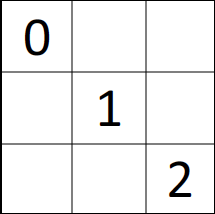
\includegraphics[scale=0.25]{sudoku-3.png}
\caption{Example of partial Latin Square of order 3.}
\end{figure}

\begin{figure}[H]
\label{fig:partialNP}
\centering
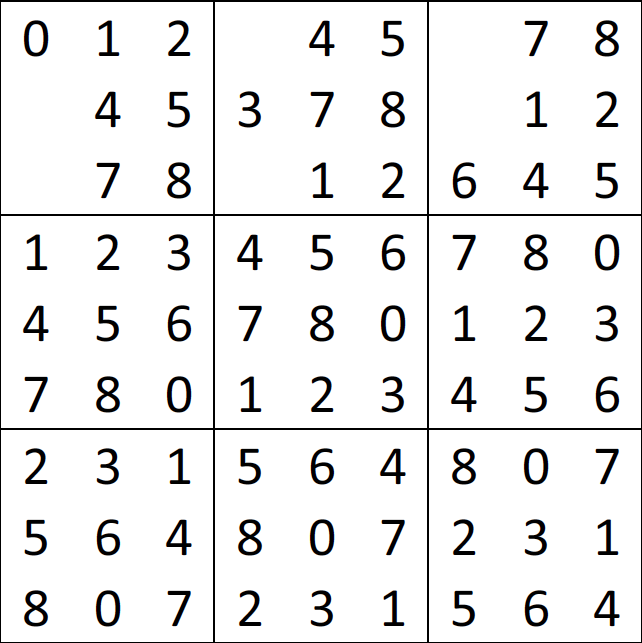
\includegraphics[scale=0.25]{sudoku-1.png}
\caption{Example of corresponding partial Number Place on a board of order 3.}
\end{figure}

\end{proof}

\section{Relationship to Other Complexity Classes.}
\label{sec:relationship}

In this section, we consider how $\mathsf{FCP}$ fits in relation to the well-known complexity classes, $\mathsf{NP}, \mathsf{coNP}, \mathsf{NP}^\mathsf{NP}, \mathsf{PSPACE}$. Recall that $\mathsf{NP}^\mathsf{NP}$ refers to the class of problems solvable in nondeterministic polynomial time with an $\mathsf{NP}$-oracle. We give a number of different containments, but it remains to be shown if any of these containments are strict.

\begin{proposition}
$\NP \subset \mathsf{FCP}$
\end{proposition}

\begin{proof}
If a problem is in $\NP$, then there exists an NTM which decides in time at most $p(n)$, where $p$ is a polynomial and $n$ is the size of the input. Thus, we can solve any problem in $\NP$ with the following equivalent $\mathsf{FCP}$ question: is there a partial (possibly full) certificate of size at most $p(n)$?
\end{proof}

\begin{corollary}
If a problem is $\mathsf{FCP}$-hard, it is also $\NP$-hard.
\end{corollary}

\begin{proposition}
If a problem is $\mathsf{FCP}$-hard, it is also $\coNP$-hard. 
\end{proposition}

\begin{proof}
Consider the problem of $\mathsf{UNIQUE-SAT}$, which gives a Boolean formula and asks if there is exactly one solution. This problem is known to be $\coNP$-hard \cite{blass1982unique}. We can solve $\mathsf{UNIQUE-SAT}$ by asking the following $\mathsf{FCP}$ question: given a Boolean formula, is there a partial certificate of size at most 0? If and only if such a certificate exists, then by definition of the Boolean formula is uniquely satisfiable.
\end{proof}

We switch our focus now to the problem of $\mathsf{FCP-SAT}$, an $\mathsf{FCP}$-complete problem. 

\begin{proposition}
$\mathsf{FCP}$ is contained in $\NP^{\NP}$.
\end{proposition}

\begin{proof}
We do this by providing an algorithm that solves $\mathsf{FCP-SAT}$ with an NTM with a SAT oracle. 

The algorithm we give will rely on the following observations.

\textbf{Observation 1:} A Boolean formula $\phi$ has a partial assignment of $k$ variables which yield a unique solution if and only if for every variable outside the partial assignment, one assignment of this variable yields a satisfiable formula, and the other does not. This observation holds due to the fact that there is only one accepting branch.

\textbf{Observation 2:} A Boolean formula $\phi$ with a partial assignment of $k$ variables is \emph{not} uniquely satisfiable if and only if there exists a variable outside of the partial assignment for which both truth assignmetns of this variable give a satisfiable Boolean formula. This observation holds because this situation corresponds exactly with cases where we are not on a unique accepting branch.

To complete the proof, we simply give the algorithm:

\begin{codebox}
\Procname{$\mathsf{FCP-SAT}$: Instance: $\phi$ formula with variables $\{ x_i \}$ and variable $k$.}
\li \For $i = 1, ..., k$ \Then
\li Non-deterministically pick a variable $x_i$, without repetition
\li Non-deterministically pick an assignment \End
\li Iterate through all remaining variables \Then
\li \If a variable is such that both assignments give a satisfiable formula \Then
\li reject
\li \Else assign that variable \End \End
\li Once you have assigned all variables, accept.
\end{codebox}
\end{proof}


\section{Conclusion}
\label{sec:conclusion}

We have formalized the notion of what it means for a problem to be uniquely solvable after giving the fewest possible number of clues. This gave rise to the $\mathsf{FCP}$ class. We presented $\mathsf{FPC}$ versions of some classical $\NP$ problems and showed they were complete for this class. In particular, this means $\mathsf{FCP-Sudoku}$ is $\NP$-hard, but is unlikely to be $\PSPACE$-hard. However, the instances of $\mathsf{FCP-Sudoku}$ which make it $\mathsf{FCP}$-complete are very far from empty. In fact, just by looking at the last reduction from $\mathsf{FCP-Latin Squares}$, a Sudoku of dimensions $n^2 \times n^2$ which is a hard instance, at most $n^2$ of the $n^4$ squares at empty. It would be interesting to see if the empty instances of Sudoku are still complete for $\mathsf{FCP}$. This would be exactly the problem \cite{mcguire2012there} solved for $n = 3$. 

Further work in the field includes looking at other related results and adapting our framework to a the more general setting. The authors also think that it is important to determine where this class fits in the complexity zoo. In particular, there seem to be connections with the class $\#P$. A stricter notion of a reduction might also be required. Finally, it would be interesting to find problems in $\P$ such that their $\mathsf{SPC}$ versions are as hard for the class, or $\NP$ hard problems such that their $\mathsf{SPC}$ versions are not hard for the class. 

\bibliography{references}
\bibliographystyle{splncs}
\end{document}
